\documentclass[journal, a4paper]{IEEEtran}
\usepackage[T1]{fontenc}       % Encodage le plus étendu
\usepackage[utf8]{inputenc}    % Source Unicode en UTF-8

\usepackage[cyr]{aeguill}
\usepackage[francais]{babel} % Pour la redaction du document en francais


% some very useful LaTeX packages include:

%\usepackage{cite}      % Written by Donald Arseneau
                        % V1.6 and later of IEEEtran pre-defines the format
                        % of the cite.sty package \cite{} output to follow
                        % that of IEEE. Loading the cite package will
                        % result in citation numbers being automatically
                        % sorted and properly "ranged". i.e.,
                        % [1], [9], [2], [7], [5], [6]
                        % (without using cite.sty)
                        % will become:
                        % [1], [2], [5]--[7], [9] (using cite.sty)
                        % cite.sty's \cite will automatically add leading
                        % space, if needed. Use cite.sty's noadjust option
                        % (cite.sty V3.8 and later) if you want to turn this
                        % off. cite.sty is already installed on most LaTeX
                        % systems. The latest version can be obtained at:
                        % http://www.ctan.org/tex-archive/macros/latex/contrib/supported/cite/

\usepackage{graphicx}   % Written by David Carlisle and Sebastian Rahtz
                        % Required if you want graphics, photos, etc.
                        % graphicx.sty is already installed on most LaTeX
                        % systems. The latest version and documentation can
                        % be obtained at:
                        % http://www.ctan.org/tex-archive/macros/latex/required/graphics/
                        % Another good source of documentation is "Using
                        % Imported Graphics in LaTeX2e" by Keith Reckdahl
                        % which can be found as esplatex.ps and epslatex.pdf
                        % at: http://www.ctan.org/tex-archive/info/

%\usepackage{psfrag}    % Written by Craig Barratt, Michael C. Grant,
                        % and David Carlisle
                        % This package allows you to substitute LaTeX
                        % commands for text in imported EPS graphic files.
                        % In this way, LaTeX symbols can be placed into
                        % graphics that have been generated by other
                        % applications. You must use latex->dvips->ps2pdf
                        % workflow (not direct pdf output from pdflatex) if
                        % you wish to use this capability because it works
                        % via some PostScript tricks. Alternatively, the
                        % graphics could be processed as separate files via
                        % psfrag and dvips, then converted to PDF for
                        % inclusion in the main file which uses pdflatex.
                        % Docs are in "The PSfrag System" by Michael C. Grant
                        % and David Carlisle. There is also some information
                        % about using psfrag in "Using Imported Graphics in
                        % LaTeX2e" by Keith Reckdahl which documents the
                        % graphicx package (see above). The psfrag package
                        % and documentation can be obtained at:
                        % http://www.ctan.org/tex-archive/macros/latex/contrib/supported/psfrag/

%\usepackage{subfigure} % Written by Steven Douglas Cochran
                        % This package makes it easy to put subfigures
                        % in your figures. i.e., "figure 1a and 1b"
                        % Docs are in "Using Imported Graphics in LaTeX2e"
                        % by Keith Reckdahl which also documents the graphicx
                        % package (see above). subfigure.sty is already
                        % installed on most LaTeX systems. The latest version
                        % and documentation can be obtained at:
                        % http://www.ctan.org/tex-archive/macros/latex/contrib/supported/subfigure/

\usepackage{url}        % Written by Donald Arseneau
                        % Provides better support for handling and breaking
                        % URLs. url.sty is already installed on most LaTeX
                        % systems. The latest version can be obtained at:
                        % http://www.ctan.org/tex-archive/macros/latex/contrib/other/misc/
                        % Read the url.sty source comments for usage information.

%\usepackage{stfloats}  % Written by Sigitas Tolusis
                        % Gives LaTeX2e the ability to do double column
                        % floats at the bottom of the page as well as the top.
                        % (e.g., "\begin{figure*}[!b]" is not normally
                        % possible in LaTeX2e). This is an invasive package
                        % which rewrites many portions of the LaTeX2e output
                        % routines. It may not work with other packages that
                        % modify the LaTeX2e output routine and/or with other
                        % versions of LaTeX. The latest version and
                        % documentation can be obtained at:
                        % http://www.ctan.org/tex-archive/macros/latex/contrib/supported/sttools/
                        % Documentation is contained in the stfloats.sty
                        % comments as well as in the presfull.pdf file.
                        % Do not use the stfloats baselinefloat ability as
                        % IEEE does not allow \baselineskip to stretch.
                        % Authors submitting work to the IEEE should note
                        % that IEEE rarely uses double column equations and
                        % that authors should try to avoid such use.
                        % Do not be tempted to use the cuted.sty or
                        % midfloat.sty package (by the same author) as IEEE
                        % does not format its papers in such ways.

\usepackage{amsmath}    % From the American Mathematical Society
                        % A popular package that provides many helpful commands
                        % for dealing with mathematics. Note that the AMSmath
                        % package sets \interdisplaylinepenalty to 10000 thus
                        % preventing page breaks from occurring within multiline
                        % equations. Use:
%\interdisplaylinepenalty=2500
                        % after loading amsmath to restore such page breaks
                        % as IEEEtran.cls normally does. amsmath.sty is already
                        % installed on most LaTeX systems. The latest version
                        % and documentation can be obtained at:
                        % http://www.ctan.org/tex-archive/macros/latex/required/amslatex/math/

\usepackage{lipsum} % Dummy text


% Other popular packages for formatting tables and equations include:

%\usepackage{array}
% Frank Mittelbach's and David Carlisle's array.sty which improves the
% LaTeX2e array and tabular environments to provide better appearances and
% additional user controls. array.sty is already installed on most systems.
% The latest version and documentation can be obtained at:
% http://www.ctan.org/tex-archive/macros/latex/required/tools/

% V1.6 of IEEEtran contains the IEEEeqnarray family of commands that can
% be used to generate multiline equations as well as matrices, tables, etc.

% Also of notable interest:
% Scott Pakin's eqparbox package for creating (automatically sized) equal
% width boxes. Available:
% http://www.ctan.org/tex-archive/macros/latex/contrib/supported/eqparbox/

% *** Do not adjust lengths that control margins, column widths, etc. ***
% *** Do not use packages that alter fonts (such as pslatex).         ***
% There should be no need to do such things with IEEEtran.cls V1.6 and later.


% En-tête et pied de page
%\usepackage{lastpage}
%\usepackage{fancyhdr}
%\pagestyle{fancy}
%\renewcommand{\sectionmark}[1]{\markright{#1}}
%\fancyhead{}
%%\fancyhead[RO,LE]{\slshape\footnotesize\nouppercase{\rightmark}}
%\fancyhead[LO,RE]{\thetitle}
%\fancyfoot{}
%%\fancyfoot[LO,RE]{\footnotesize\texttt{\thefilename}\\ \textit{\now}}
%%\fancyfoot[C]{-~\thepage~/~\pageref{LastPage}~-}
%\fancyfoot[RO,LE]{\raisebox{-2mm}{\includegraphics{structure/barrette-original}}}
%%
%\fancypagestyle{plain}{ %  Première page ----------------------
%  \fancyhead{}
%  \renewcommand{\headrulewidth}{0pt}
%  \fancyheadoffset[R]{15mm}
%  \fancyhead[L]{
%    \raisebox{-7mm}{
%      \parbox{\textwidth}{
%        \includegraphics{structure/barrette-original} \\ \\
%        \fontsize{8pt}{10pt}\selectfont
%        \sffamily\color{Pantone287}
%        FACULTÉ DES SCIENCES       \\
%        DÉPARTEMENT D'INFORMATIQUE
%      }
%    }
%  }
%  \fancyhead[R]{
%    \raisebox{-10mm}[0pt][0pt]{\includegraphics[width=120mm]{structure/ULB-ligne-gauche}}
%  }
%  \fancyfoot{}
%  %\fancyfoot[L]{\raisebox{0mm}{}\color{Pantone287}\footnotesize\texttt{\thefilename}\\ \textit{\now}}
%  %\fancyfoot[C]{-~\thepage~/~\pageref{LastPage}~-}
%  \fancyfoot[R]{
%    \raisebox{-12pt}{\includegraphics[height=\footskip]{structure/sceau-mini-b-quadri}}
%  }
%} % Fin de première page
% ---------------------------------------------------------------------------


% Your document starts here!
\begin{document}

% Define document title and author
	\title{Modélisation de la vaccination des individus et de la population dans le cadre d'une épidémie}
	\author{Nathan Marotte
	\thanks{Superviseurs: Robin Petit}}
	\markboth{INFO-F308}{}
	\maketitle

% Write abstract here
\begin{abstract}
	Le vaccin est un sujet souvent débattu car son efficacité n'est pas ressentie de la même manière qu'un antibiotique ou qu'un anti-douleur. Nous allons montrer dans cet article, par des modèles et simulations simple, comment un vaccin altère la propagation d'une maladie, au-delà de la protection qu'il apporte à un individu, en créant une véritable barrière qui rend la population immunisée si un certain pourcentage de la population est vacciné.
	Le résumé (80-100 mots) est conçu pour donner au lecteur une vue générale sur le contenu de l'article.
\end{abstract}

% Each section begins with a \section{title} command
\section{Introduction}
	% \PARstart{}{} creates a tall first letter for this first paragraph
	\PARstart{L}{e} monde étant rempli de sceptiques, les vaccins ont reçu et reçoivent encore bon nombre de critiques sur leur efficacité et donc autant de personnes refusant de ce faire vacciner. Les taux d'exemptions non médicales des vaccins varient d'une population à l'autre mais aurait atteint jusque 26.67\% \cite{NME_vaccine} dans certaines populations. Comme nous le verrons plus loin, toutes ces personnes contribuent à une augmentation du risque d'épidémie, un anéantissement du phénomène d'immunité collective, et mettent en danger la vie des individus ne pouvant pas être vaccinés pour raisons médicales.\

	Cet article aura donc pour but de défendre la vaccination en simulant la propagation d'une épidémie dans une population vaccinée à un certain pourcentage afin de voir comment le taux de vaccination dans une population influence de manière \emph{non linéaire} l'immunité de la maladie. Cette relation est aussi connue sous le nom d'immunité grégaire ou \emph{herd immunity, en anglais}.
	Trouver le seuil de cette immunité, c'est-à-dire le taux de vaccination nécéssaire pour que la maladie se propage moins vite que l'on en guérit, permettra de déterminer quelles populations sont potentiellement en danger d'épidémies graves, et de pouvoir nous concentrer sur celles-ci afin d'éviter d'autres catastrophes. Ce seuil est appellé \emph{Herd Immunity Threshold}, ou \emph{HIT}
	Notre approche fournira à la communauté scientifique des méthodes très simples et compréhensibles, mais correctes pour démontrer au public les raisons de la vaccination obligatoire.

\section{Etat de l'art}
	Le modèle étant par nature assez simple, peu d'articles récents ont été écrits sur le sujet. Par contre, il existe déjà plusieurs expériences ayant été réalisées notamment des simulations sur la propagation de la grippe saisonnière \cite{pandemic_influenza} \cite{influenza_HIT}, ainsi que sur le VIH \cite{VIH}. Ces expériences utilisent pour la plupart un modèle similaire à SIR qui sera donc aussi utilisé pour modéliser notre problème

% Main Part
\section{Méthodologie}\label{sec:met}
	Afin d'étayer notre hypothèse, les vaccins protègent au delà du système immunitaire, nous avons construit un modèle SIR simple où la population de départ est repartie dans les différents états pour une représentation compartimentale et nous avons aussi construit une modèle spatial se basant sur les 3 états et les transitions du modèle compartimental SIR.
	Grâce à ces modèles, nous allons pouvoir déterminer le seuil d'immunité grégaire \emph{HIT} mais aussi voir l'évolution de la protection en fonction du nombre de vaccinés.
	\subsection{Modèle SIR}
	Notre modèle SIR est composé de 3 états et de une transition disposée comme dans la figure \ref{fig:MySIR}

	\begin{figure}
		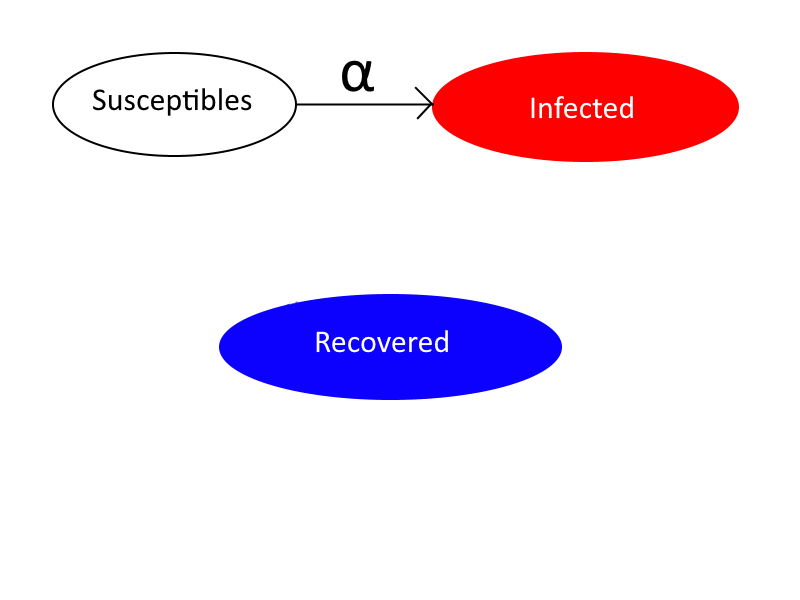
\includegraphics[scale=0.4]{MySIR}
		\caption{Modèle SIR}
		\label{fig:MySIR}
	\end{figure}


	Ces états, susceptibles, infectés, et retirés, représentent respectivement la population saine, la population malade et contagieuse, et la population vaccinée. $\alpha$ représente la probabilité qu'un individu sain se fasse infecté.
	Ce modèle seul ne permet pas de simuler de manière satisfaisante et représentative l'évolution dans une population, nous l'avons donc adapté dans un modèle spatial décrit en \ref{sec:modele_spatial}

	\subsection{Modèle spatial}
	\label{sec:modele_spatial}
	Ce modèle se base sur la représentation d'une population de 2500 individus sur un plan en 2 dimensions. Chaque individu est représenté par un point sur une matrice carrée de 50 points de côtés, ne peut être dans un état à la fois, et est voisin de 8 autres individus. Un individu ne peut infecter que quelqu'un dont il est voisin. Un malade contagieux ne pourra donc pas infecter plus de 8 individus ($R_0 = 8$)
	D'abord tous les individus commencent susceptibles, puis, avant le début de l'infection, une proportion fixée de la population est vacciné, puis, une personne au hasard est sélectionnée pour être l'infecté de départ (Le programme Python que nous avons écrit permet de faire varier ces paramètres)
	\subsubsection{L'infection de départ}
	Parmi les personnes saines dans la population, nous sélectionnons une personne au hasard pour démarrer l'épidémie
	\subsubsection{La propagation}
	Pour chaque voisin susceptible de chaque individu infecté, nous l'infectons avec une probabilité de $\alpha$. Dans le cadre de ce projet, nous avons choisi un $\alpha$ de $1$ car nous voulions voir l'évolution d'une maladie très infectieuse, évoluant donc rapidement avec le temps. Choisir une valeur de $\alpha < 1$ ne serait pas utile dans cette étude étant donné qu'il n'y a que une transition dans le modèle, diminuer le taux de transition revient donc simplement à ralentir la simulation.
	\subsubsection{Probabilité de propagation et isolement}
	Au vu de la construction de notre modèle spatiale, il existe des cas particuliers empêchant totalement la propagation de la maladie, par exemple si un individu est entouré de 8 individus vacciné.
	Ces individus sont donc totalement protégés du fait qu'ils n'ont aucun voisins capable de leur transmettre la maladie. En fonction du pourcentage de vaccination de la population, le nombre d'individus isolé augmente.
	Aussi, chaque voisin vacciné autour d'un individu susceptible diminue au final la probabilité de cet individu d'être infecté. Si la maladie vient de la direction dans laquelle l'individu susceptible a son voisin vacciné, elle mettra plus de temps à l'atteindre, cette durée supplémentaire augmente les chances que la maladie s'arrête dû au fait que un des infecté guérisse ou meurt, épargnant alors de justesse l'individu susceptible.
	La probabilité qu'un individu ai k voisins vaccinés est représentée en \ref{fig:probNeighbour}
	Cette probabilité est calculée en utilisant une binomiale. En effet, la probabilité d'avoir k voisins vacciné lorsque la probabilité d'être vacciné est de p, est égale au fait de réussir k événement ``recevoir un vaccin'' en n (nombre de voisins) tentatives avec une probabilité de p de réussite de l'événement. Nous avons donc
	\begin{equation}
	\begin{aligned}
		P(X = k) = B(n;p) = {n \choose k}\times p^k \times (1-p)^{n-k} = \\ \frac{n!}{k!(n-k)!}\times p^k \times (1-p)^{n-k}
	\end{aligned}
	\end{equation} où X est la variable aléatoire ``Nombre de voisins vaccinés'', k le nombre de voisins vaccinés (entre 1 et 8), p la probabilité pour un individu d'être vacciné, et n le nombre de voisins, 8 dans notre simulation. En calculant cette valeur pour tous les pourcentages de vaccination et pour tous les nombres de voisins vaccinés de 1 à 8, nous obtenons ce graphe

	\begin{figure}
		\caption{Probabilité d'avoir x voisins vaccinés en fonction du pourcentage de vaccinés}
		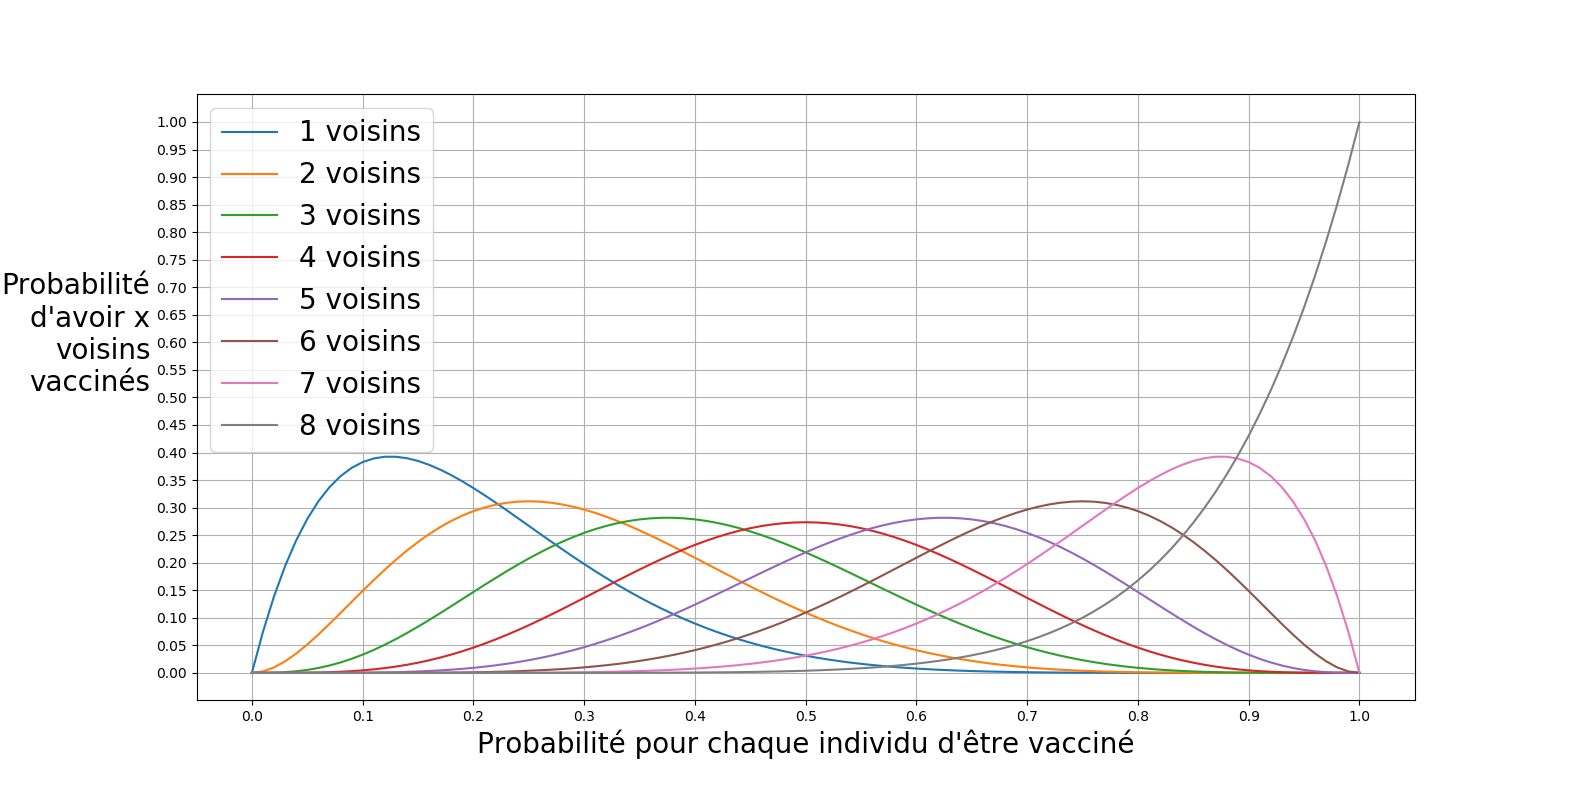
\includegraphics[scale=0.2]{probNeighbour}
		\label{fig:probNeighbour}
	\end{figure}

	Nous voyons donc que lorsque la population est vaccinée à 90\%, il y a déjà plus de 40\% des individus qui sont totalement isolés de la maladie. Il s'agit donc de 40\% d'individus qui n'attraperont jamais la maladie ce qui réduit automatiquement le taux de personnes infecté à la fin de l'épidémie. Cette immunité par isolement n'apporte malheureusement que trop peu de protection que pour être considéré comme un moyen efficace de protéger la population.

	\subsubsection{Seuil d'Immunité Grégaire (HIT)}
	Ce seuil d'immunité est dépend de $R_0$, le nombre d'individus qu'un malade infecte en moyenne. Si ce nombre est inférieur à 1, alors la maladie finira par s'éteindre, si il est supérieur à 1, la maladie infectera tout le monde si rien n'est fait pour l'arrêter.
	Le taux de reproduction effectif, noté $R_t = R_0 \times (1-P)$ quant à lui est une mesure du nombre d'individu qu'un malade infecte au temps t, c'est-à-dire en tenant compte des ``barrières''(vaccins), mais aussi de la mortalité et de la virulence de la maladie. $P$ est la proportion d'individus vaccinés. Le taux de reproduction effectif $R_t$ sera inférieur à 1 pour autant que la valeur de P soit supérieure à $1-1/R_0$. Un individu malade contaminera alors en moyenne moins d'une personne ce qui finira par faire tomber le nombre de malades à 0 pour peu que les malades guérissent ou meurt. Il faut donc vacciner une proportion de la population égale à $1-\frac{1}{R_0}$ pour qu'un malade ne puisse plus infecter, en moyenne, qu'une personne dans son entourage.\\
	Dans le cadre de notre modèle, ce taux est donc de $0.875$. Ce qui signifie que, en moyenne, dans une population infinie, si chaque individu est vacciné avec une probabilité de 0.875, la maladie se transmettrait un individu à la fois et ne s'arrêterait que lorsque toute la population aura été touchée. A $0.875+\epsilon$ de la population vaccinée, la maladie se hurterait à un moment sur une personne qui n'a aucun voisin susceptible et s'arrêtera donc là. Plus $\epsilon$ est grand, plus ce moment arrivera vite après l'infection du patient zéro

	Afin de détecter une protection des vaccins au-delà de l'individu, nous avons donc écrit un programme Python qui va générer 500.000 populations de 2500 individus chacun. Chaque population aura un taux de vaccination de telle sorte qu'il y aura 5000 populations par pourcentage de vaccination (entre 0 et 99\%). Ensuite nous faisons la moyenne du nombre de personnes qui n'étaient pas vaccinés et qui n'ont pas été touchées par la maladie (en excluant des calculs le patient zéro), en regroupant les populations par taux de vaccination.

% Main Part
\section{Résultats}
	Nous obtenons ainsi une courbe en S liant le taux de vaccination, sur l'axe des abscisses, au taux de protection des individus non-vaccinés, sur l'axe des ordonées sur la figure \ref{fig:results}.
	\begin{figure}
	\caption{Efficacité de la couverture vaccinale sur les individus non vaccinés}
		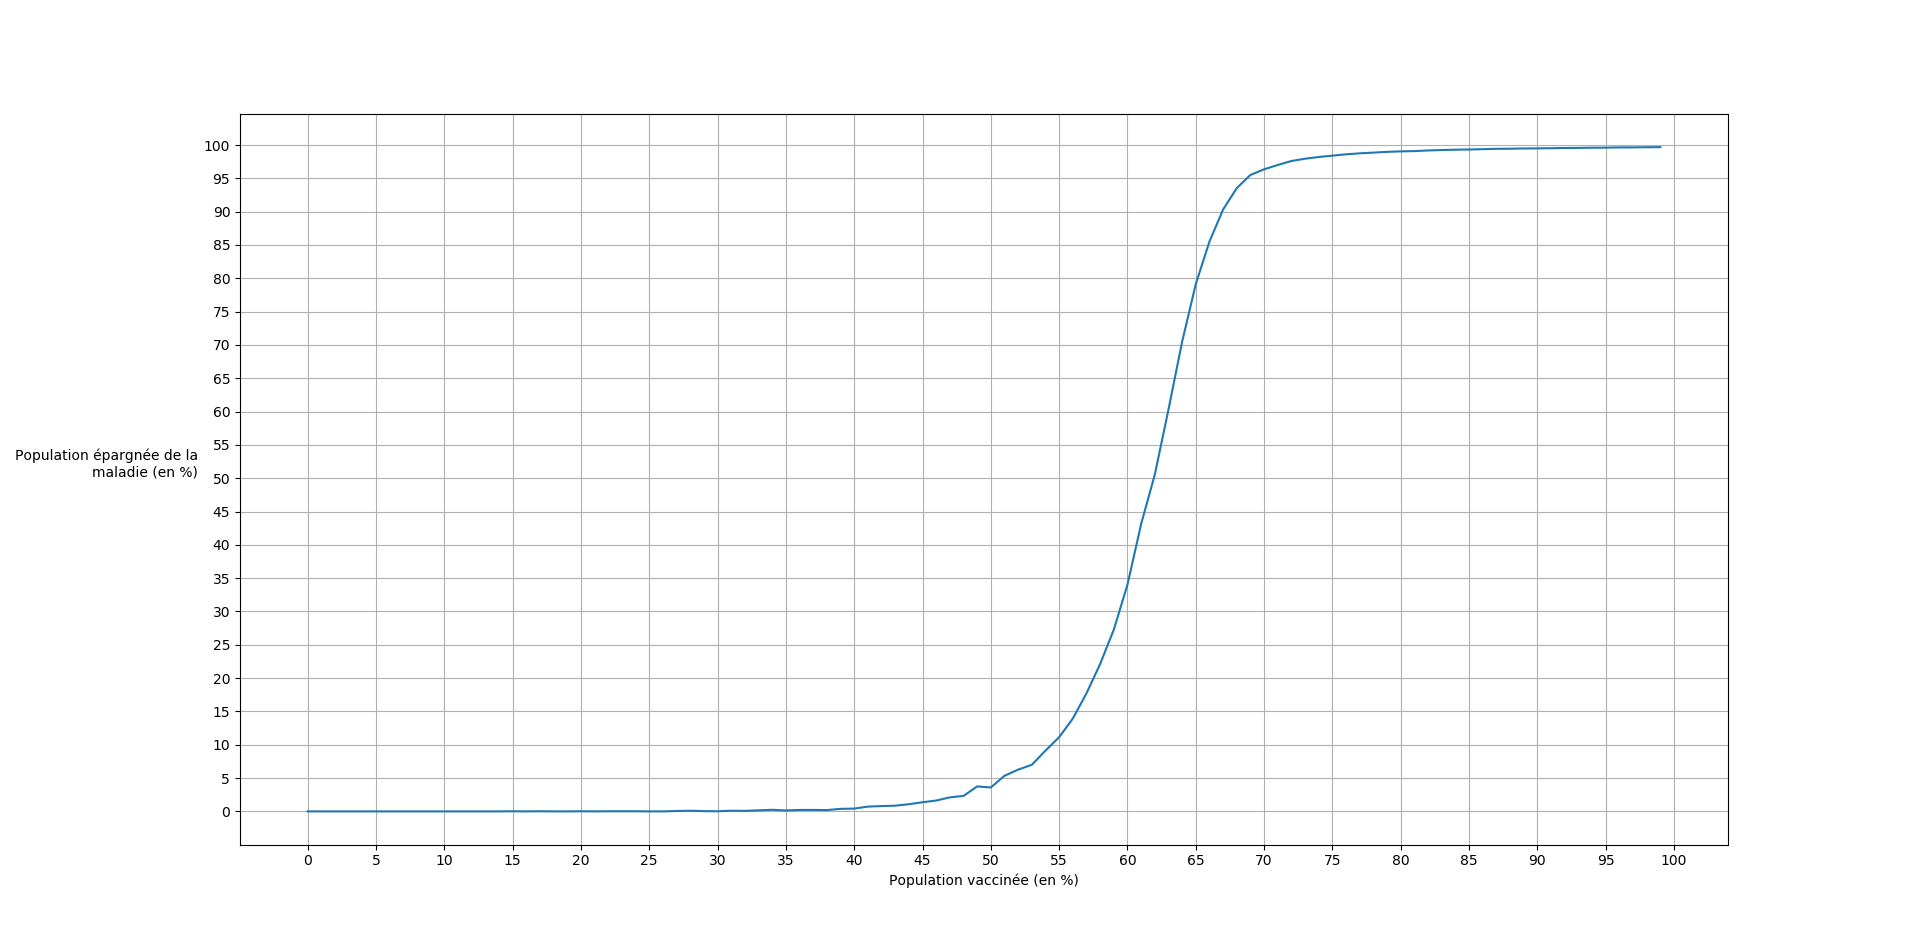
\includegraphics[scale=0.2]{Results}
		\label{fig:results}
	\end{figure}
	Cette courbe est assez remarquable. On remarque que vacciner une population à seulement environ 40\% est inneficace pour empêcher une maladie de se répandre. Par contre, entre 40 et 75\%, chaque personne vacciné compte au vu de la croissance ultra-rapide de la courbe entre ces deux valeurs. Enfin on peut aussi remarquer qu'à
	% Cette section doit contenir les résultats que vous avez obtenu avec la méthodologie décrite dans la section \ref{sec:met}.
	% Les résultats devront être présentés de préférence sous forme de tableau (cf. Table~\ref{tab:simParameters}) et/ou du diagramme (cf. Fig.~\ref{fig:tf_plot}), et correctement référencés.
	% Le conditions d'expérimentation (c-à-d matériel et logiciels utilisés) devront être ainsi indiquées.
	% En plus des résultats mêmes, cette section devra contenir votre propre analyse et discussion de résultats (par example comparaison par rapport à une méthode de référence)

% This is how you define a table: the [!hbt] means that LaTeX is forced (by the !) to place the table exactly here (by h), or if that doesnt work because of a pagebreak or so, it tries to place the table to the bottom of the page (by b) or the top (by t).
	% \begin{table}[!hbt]
	% 	% Center the table
	% 	\begin{center}
	% 	% Title of the table
	% 	\caption{Simulation Parameters}
	% 	\label{tab:simParameters}
	% 	% Table itself: here we have two columns which are centered and have lines to the left, right and in the middle: |c|c|
	% 	\begin{tabular}{|c|c|}
	% 		% To create a horizontal line, type \hline
	% 		\hline
	% 		% To end a column type &
	% 		% For a linebreak type \\
	% 		Information message length & $k=16000$ bit \\
	% 		\hline
	% 		Radio segment size & $b=160$ bit \\
	% 		\hline
	% 		Rate of component codes & $R_{cc}=1/3$\\
	% 		\hline
	% 		Polynomial of component encoders & $[1 , 33/37 , 25/37]_8$\\
	% 		\hline
	% 	\end{tabular}
	% 	\end{center}
	% \end{table}

	% This is how you include a eps figure in your document. LaTeX only accepts EPS or TIFF files.
	% \begin{figure}[!hbt]
	% 	% Center the figure.
	% 	\begin{center}
	% 	% Include the eps file, scale it such that it's width equals the column width. You can also put width=8cm for example...
	% 	%\includegraphics[width=\columnwidth]{plot_tf}
	% 	% Create a subtitle for the figure.
	% 	\caption{Simulation results on the AWGN channel. Average throughput $k/n$ vs $E_s/N_0$.}
	% 	% Define the label of the figure. It's good to use 'fig:title', so you know that the label belongs to a figure.
	% 	\label{fig:tf_plot}
	% 	\end{center}
	% \end{figure}

\section{Conclusion}
TODO
% Cette section contient un rappel des contributions / de résultats importants de votre article et éventuellement une indication sur les perspectives de recherche future dans le même domaine.


\bibliographystyle{unsrt}
\bibliography{bibliography}

\newpage

\appendices
\section{Consignes}
% Main Part
\subsection*{Document}
	% LaTeX takes complete care of your document layout ...
	% Le rapport doit être rédigé en \LaTeX{} suivant ce template.
	% La longueur du rapport ne devra pas, en tout cas, dépasser les 6 pages.
	% Ce rapport doit être \emph{self-contained}, c-à-d il doit pouvoir être lu et compris sans avoir besoin de se documenter ailleurs.



% Your document ends here!
\end{document}
